% ============================================================
% Amazon-VT Fellowship Application 2026-2027
% AKG-E: A Doctoral Research Vision with Simulation-Grounded Validation
% Applicant: Jason Cusati (PhD Candidate, Virginia Tech)
% Advisor:   Chris Brown
% Primary:   AI Accelerated Science & Engineering
% Secondary: Agentic AI
% Format:    IEEE 2-column, 2 pages + references
% Note:      Hybrid of abstract_v4e research vision +
%            net-new student-centric personal-statement sections.
% ============================================================

\documentclass[conference, 10pt]{IEEEtran}

\usepackage[utf8]{inputenc}
\usepackage[T1]{fontenc}
\usepackage{graphicx}
\usepackage{hyperref}
\usepackage{microtype}
\usepackage{cite}
\usepackage{enumitem}
\setlist{nosep, leftmargin=1.5em, topsep=0.2em}
\usepackage{tikz}
\usetikzlibrary{positioning, arrows.meta, shapes.geometric, fit, calc}

\title{Agentic Knowledge Graphs for AI-Accelerated Engineering: \\
       A Doctoral Research Vision with Simulation-Grounded Validation}
\author{
    \IEEEauthorblockN{Jason Cusati}\\
    \IEEEauthorblockA{PhD Candidate, Virginia Tech \\
    Advisor: Chris Brown}
}
\date{}

\begin{document}

\maketitle
\thispagestyle{empty}

\vspace{-1.5em}

\noindent\textbf{Primary Topic:} AI Accelerated Science \& Engineering \hfill
\textbf{Secondary:} Agentic AI

\vspace{0.5em}

\section*{Research Vision and Motivation}

My doctoral research investigates how agentic AI systems can be coupled with structured engineering knowledge and physics-based simulation to produce outputs that engineers can trust and deploy. The proposed research sits at the intersection of four threads I have been actively working on at Virginia Tech: (i)~an agentic knowledge-graph system for research progression that models scientific problems and constraints as first-class entities; (ii)~a knowledge-graph and computer-vision toolset of my own design for automated construction material takeoff, whose output feeds into Dr.~Kereshmeh Afsari's construction.ai 3D-visualization tooling; (iii)~the Virginia Transportation Safety Index, where I built an initial real-time safety-index calculator over multimodal-sensor data at the Virginia Tech Transportation Institute (VTTI), with a follow-on proposal extending the work to a digital-twin formulation with formal verification; and (iv)~graduate coursework with Dr.~Christopher Roy on the Oberkampf--Roy Verification, Validation, and Uncertainty Quantification (VVUQ) formulation~\cite{Oberkampf2010VVUQ}, which supplies the disciplinary foundation for trusting computational outputs. AKG-E is the synthesis: domain knowledge graphs and simulators below, agent orchestration above, and a VVUQ validation layer that turns generative outputs into certified, decision-ready engineering artifacts. Studying how generative tools handle (and mishandle) evidence-based reasoning~\cite{Ji2023HallucinationSurvey}---joint work with my advisor Dr.~Chris Brown---sharpened the central concern: large language models can describe a beam, but they cannot certify that it will hold, and engineering disciplines reject what they cannot verify. The Amazon-VT Fellowship would let me dedicate the next year to closing that verification gap directly, in a setting that combines academic rigor with industry-scale infrastructure.

\section*{Research Problem}

AI-driven scientific breakthroughs increasingly couple learned models with structured knowledge and simulation~\cite{Abramson2024AlphaFold3,Merchant2023GNoME}. Engineering disciplines face an analogous opportunity, yet large language models (LLMs) remain misaligned with practice: they hallucinate physical quantities, fail to enforce constraints, and lack grounding in the structured ontologies and simulation feedback loops that govern real-world systems. Knowledge-grounded generation~\cite{Lewis2020RAG,Edge2024GraphRAG} improves factual consistency but does not address the central application challenge: no established methodology validates AI-generated engineering outputs against physical laws and regulatory constraints~\cite{Oberkampf2010VVUQ}. This trust gap blocks deployment.

\section*{Approach: The AKG-E Framework}

I propose \textbf{Agentic Knowledge Graph Engineering (AKG-E)}, a domain-agnostic framework integrating knowledge-grounded reasoning with simulation-in-the-loop Verification, Validation, and Uncertainty Quantification (VVUQ), drawing on the Oberkampf--Roy formulation~\cite{Oberkampf2010VVUQ} for engineering simulation. AKG-E applies three shared layers uniformly across engineering domains, with only the domain knowledge graph and simulator swapped: (1)~a \textit{domain ontology layer} encoding engineering KGs with entities, constraints, and physical laws; (2)~a \textit{simulation integration layer} exposing domain tools (Finite Element Analysis (FEA) solvers~\cite{Logg2012FEniCS}, digital twin microsimulators~\cite{Tao2019DigitalTwin}) as typed agent-callable interfaces; and (3)~a \textit{VVUQ validation layer} that verifies outputs against governing equations, quantifies uncertainty via Monte Carlo propagation, and enforces regulatory constraints. Agents orchestrate retrieval-augmented generation, structured graph queries, and simulation feedback, extending industry knowledge-grounding approaches such as Amazon-scale KG systems~\cite{Yu2024COSMO} with physics-based validation.

\begin{figure}[t]
    \centering
    \resizebox{\columnwidth}{!}{%
    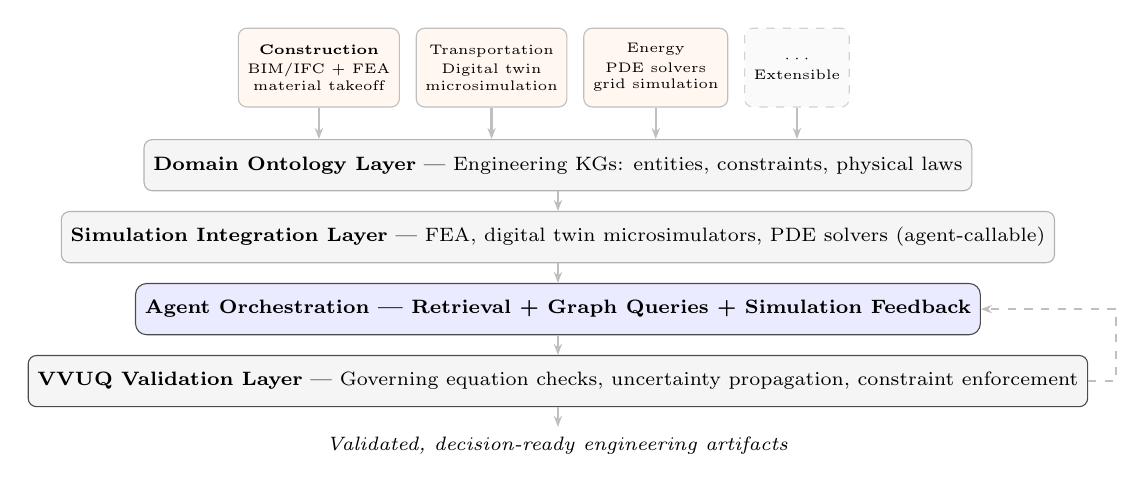
\begin{tikzpicture}[
        node distance=0.30cm and 0.20cm,
        layerbox/.style={rectangle, rounded corners=3pt, draw=gray!60, fill=gray!8, minimum width=7.8cm, minimum height=0.65cm, align=center, font=\scriptsize},
        dombox/.style={rectangle, rounded corners=3pt, draw=gray!50, fill=orange!6, minimum width=1.75cm, minimum height=1.0cm, align=center, font=\tiny},
        extbox/.style={rectangle, rounded corners=3pt, draw=gray!35, fill=gray!4, minimum width=1.05cm, minimum height=1.0cm, align=center, font=\tiny, dashed},
        agentbox/.style={rectangle, rounded corners=4pt, draw=black!70, fill=blue!8, minimum width=7.8cm, minimum height=0.65cm, align=center, font=\scriptsize\bfseries},
        arr/.style={-{Stealth[length=4pt]}, thick, gray!50},
    ]
        \node[dombox] (con) {\textbf{Construction}\\[1pt]BIM/IFC + FEA\\material takeoff};
        \node[dombox, right=0.20cm of con] (traf) {Transportation\\[1pt]Digital twin\\microsimulation};
        \node[dombox, right=0.20cm of traf] (energy) {Energy\\[1pt]PDE solvers\\grid simulation};
        \node[extbox, right=0.20cm of energy] (ext) {$\cdots$\\Extensible};

        \node[layerbox, below=0.40cm of $(con.south)!0.5!(ext.south)$] (onto) {\textbf{Domain Ontology Layer} --- Engineering KGs: entities, constraints, physical laws};

        \node[layerbox, below=0.25cm of onto] (sim) {\textbf{Simulation Integration Layer} --- FEA, digital twin microsimulators, PDE solvers (agent-callable)};

        \node[agentbox, below=0.25cm of sim] (agent) {Agent Orchestration --- Retrieval + Graph Queries + Simulation Feedback};

        \node[layerbox, below=0.25cm of agent, draw=black!70] (val) {\textbf{VVUQ Validation Layer} --- Governing equation checks, uncertainty propagation, constraint enforcement};

        \node[font=\scriptsize, below=0.25cm of val] (out) {\textit{Validated, decision-ready engineering artifacts}};

        \draw[arr] (con.south) -- (con.south |- onto.north);
        \draw[arr] (traf.south) -- (traf.south |- onto.north);
        \draw[arr] (energy.south) -- (energy.south |- onto.north);
        \draw[arr] (ext.south) -- (ext.south |- onto.north);
        \draw[arr] (onto) -- (sim);
        \draw[arr] (sim) -- (agent);
        \draw[arr] (agent) -- (val);
        \draw[arr] (val) -- (out);
        \draw[arr, dashed] (val.east) -- ++(0.35,0) |- (agent.east);
    \end{tikzpicture}
    }%
    \caption{\textbf{AKG-E Architecture.} Domain modules (Construction: primary; Transportation, Energy: extensions) plug into shared ontology, simulation, and VVUQ layers. The dashed arrow represents iterative constraint-driven refinement.}
    \label{fig:framework}
    \vspace{-0.5em}
\end{figure}

\section*{Research Questions}

The proposed research pursues two questions. \textbf{RQ1:} How can VVUQ methodology be adapted to validate AI agent-generated engineering outputs, providing quantified uncertainty bounds and enforceable physical and regulatory constraints---evaluated against a curated benchmark of engineering tasks with known ground-truth solutions? \textbf{RQ2:} Does a domain-agnostic AKG-E architecture achieve measurable reductions in constraint violation rate and task success rate across engineering domains, relative to LLM-only and RAG-only baselines~\cite{Lewis2020RAG}? The intellectual merit lies in establishing a principled VVUQ methodology for agentic AI outputs---a contribution that separates domain-specific knowledge from shared orchestration and validation logic. The construction pilot~\cite{Eastman2011BIM} is the primary testbed: agents parse Building Information Modeling (BIM) models, perform material takeoff, invoke FEA for structural verification, and iterate under VVUQ gates until load constraints and building codes are satisfied.

\section*{Training Plan and Advisor Fit}

This fellowship would fund the central year of the proposed research. My advisor, Dr.~Chris Brown, works at the intersection of generative AI and software engineering practice; our joint paper on the evidence-based reasoning behaviors of generative AI tools~\cite{BrownCusati2025SEBeliefs} exposed the same verification weaknesses that AKG-E is designed to close---making him a natural advisor for a research program that generalizes evaluation rigor from SE tools to engineering outputs. The construction-domain pilot is supported by a working collaboration with Dr.~Kereshmeh Afsari, whose construction.ai initiative provides BIM and 3D-visualization integration for the material-takeoff output of my toolset. The VVUQ methodology is grounded in graduate coursework with Dr.~Christopher Roy at VT, where I have been applying the Oberkampf--Roy formulation directly to construction-engineering homework that doubles as the AKG-E construction-pilot prototype. The fellowship's Amazon connection is equally load-bearing: AKG-E targets deployment via Amazon Bedrock Knowledge Bases~\cite{AWSBedrockHybridSearch2024}, and direct interaction with Amazon's applied AI and construction logistics teams would let me ground the framework against real engineering data pipelines rather than only academic benchmarks. My training plan for the fellowship year is to (i)~complete and validate the construction-domain implementation, (ii)~extend AKG-E to a second domain---transportation safety, building on the VTTI safety-index calculator and the digital-twin extension proposal---to evidence the domain-agnostic claim, (iii)~publish the VVUQ-agent integration methodology and benchmarks, and (iv)~present the work at venues spanning AI for engineering and the agentic AI community.

\section*{Qualifications and Trajectory}

AKG-E synthesizes four lines of prior work I have led or co-led at Virginia Tech. \textbf{(1)~Research-AI:} I am the architect of an open agentic knowledge-graph system for research progression that models scientific problems and constraints as first-class entities and supplies the orchestration substrate AKG-E reuses. \textbf{(2)~Construction-AI:} I am developing a knowledge-graph and computer-vision toolset for automated construction material takeoff---my own design and the working prototype of AKG-E's construction pilot---whose output feeds into Dr.~Afsari's construction.ai 3D-visualization tooling. \textbf{(3)~VTTI transportation safety:} for the Virginia Transportation Safety Index, I built an initial real-time safety-index calculator using multimodal-sensor data, with a follow-on proposal extending the work to a digital-twin formulation with formal verification and uncertainty quantification---the direct precursor to AKG-E's transportation domain. \textbf{(4)~VVUQ foundations:} I have been working through the Oberkampf--Roy VVUQ formulation~\cite{Oberkampf2010VVUQ} in graduate coursework with Dr.~Roy at VT, where the homework problems are themselves construction-engineering verification tasks that fold directly into AKG-E. I am also co-author with my advisor Dr.~Brown on a study of the evidence-based reasoning behaviors of generative AI tools in software engineering~\cite{BrownCusati2025SEBeliefs}, which exposed exactly the verification weaknesses AKG-E now sets out to address. I have completed VT's PhD coursework in AI-driven software engineering, knowledge-grounded generation, and applied research methods, and am positioned to dedicate the fellowship year to executing this research program rather than to coursework or qualifying-exam preparation.

\section*{Expected Impact and Deliverables}

AKG-E aims to convert generative outputs into certified, decision-ready engineering artifacts---reducing hallucinated designs, enforcing code compliance, and enabling principled human-in-the-loop thresholds. The intellectual contribution is a methodology, not a single system: by separating domain knowledge from shared orchestration and a reusable VVUQ validation layer, AKG-E gives engineering teams a template for adopting agentic AI without giving up verification rigor. As a fellow, my deliverables would include (i)~an open-source AKG-E framework with construction and transportation reference implementations; (ii)~domain-adaptable KG ontology templates and a typed simulator-tool interface specification; and (iii)~a reproducible benchmark suite of engineering tasks with ground-truth solutions and a constraint-violation evaluation harness. I set a benchmark target of $>$50\% constraint violation reduction versus unconstrained LLM baselines as an evaluation design goal. Beyond the fellowship year, the framework's Amazon-Bedrock integration path is direct: it connects AKG-E to AWS-scale engineering data pipelines and makes the contribution immediately relevant to Amazon's applied AI and construction logistics workflows.

\bibliographystyle{IEEEtran}
\bibliography{references}

\end{document}
